\documentclass[cn,pad,chinese,chinesefont=nofont]{elegantbook}
\usepackage{latexgit}
\usepackage{hyperref}
\hypersetup{
	pdftitle={洞箫演奏 - 筒音5},
    pdfauthor={雪散舞}
}
%\usepackage{showframe}
\setCJKmainfont{Source Han Serif} 
\setCJKsansfont{Source Han Sans} 
\setCJKmonofont{Source Han Mono} 
\setCJKfamilyfont{zhsong}{Source Han Serif}
\setCJKfamilyfont{zhhei}{Source Han Sans} 
\setCJKfamilyfont{zhkai}{Source Han Mono} 
\setCJKfamilyfont{zhfs}{Source Han Mono} 
\newcommand*{\songti}{\CJKfamily{zhsong}} 
\newcommand*{\heiti}{\CJKfamily{zhhei}} 
\newcommand*{\kaishu}{\CJKfamily{zhkai}} 
\newcommand*{\fangsong}{\CJKfamily{zhfs}}

\title{洞箫演奏 - 筒音5}
\author{雪散舞}
\date{\zhtoday}
\cover{dongxiao/cover.jpeg}
\logo{monk.png}
\extrainfo{清籁远喑喑,秦楼夜思深。碧空人已去,沧海凤难寻。\\杳妙和云绝,依微向水沉。还将九成意,高阁伫芳音。}
\version{\gitcommithash}

\begin{document}
\maketitle
\frontmatter
\tableofcontents
\mainmatter

\centering
\chapter{筒音做‘低音5’}
\section{指法表}
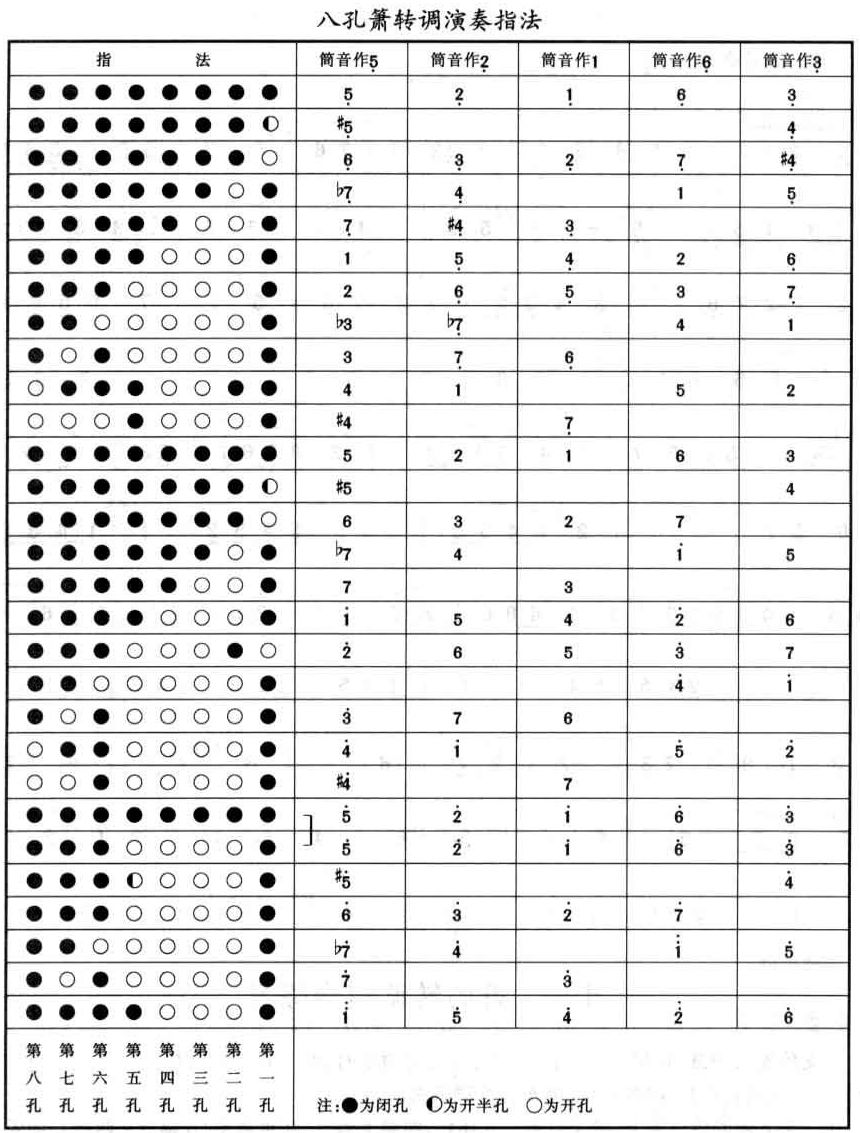
\includegraphics[width=\textwidth]{dongxiao/20200408-八孔箫指法图.jpg}
\section{世上只有妈妈好}
	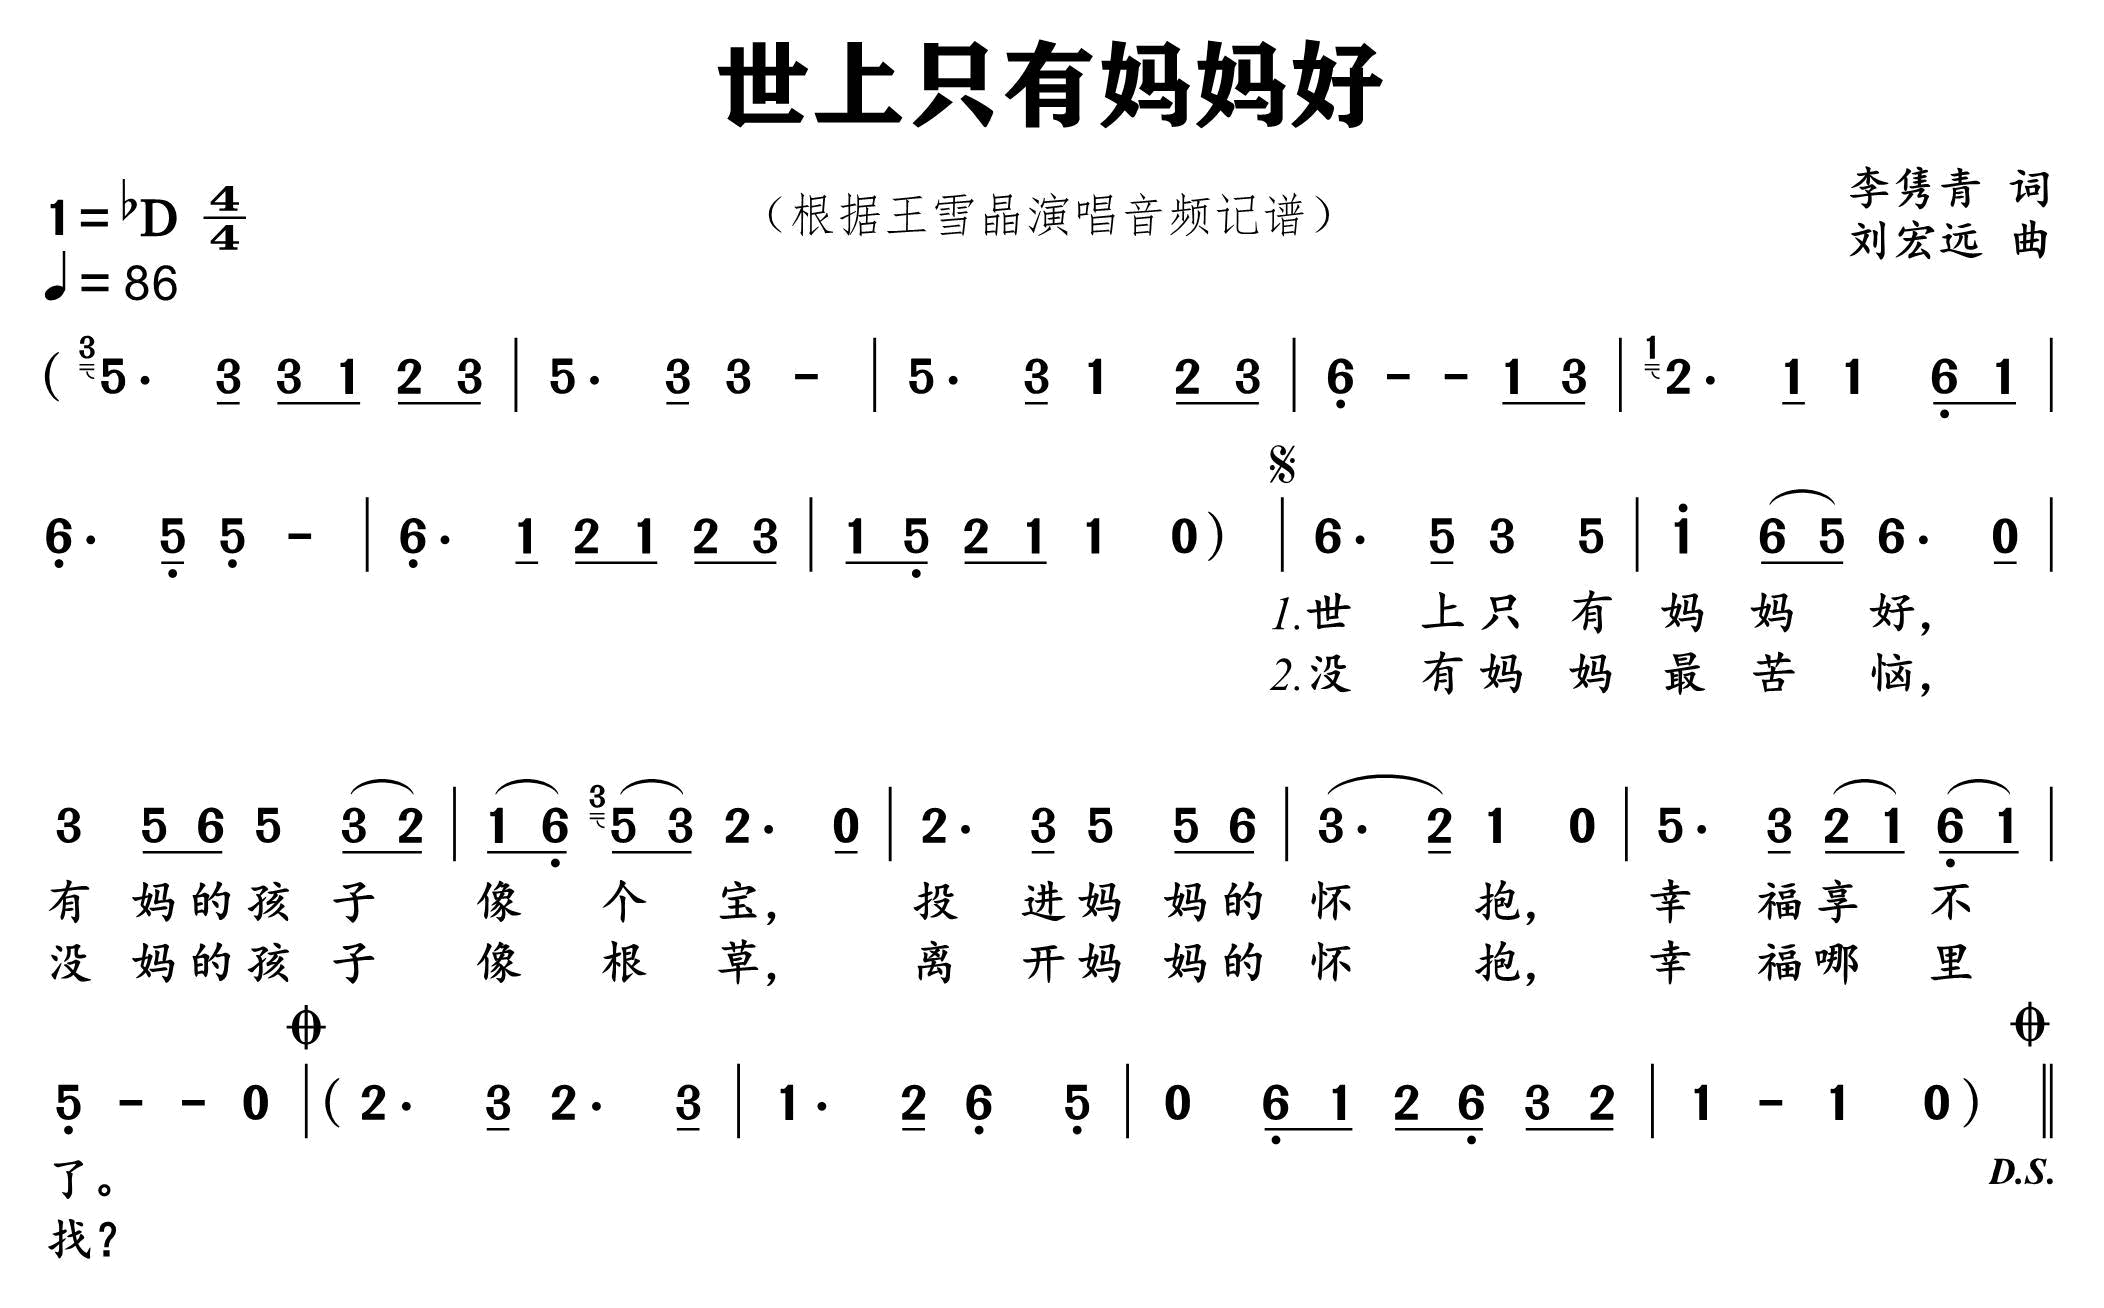
\includegraphics[width=\textwidth]{dongxiao/IMG_0854-世上只有妈妈好.png}
\section{西湖春}          
	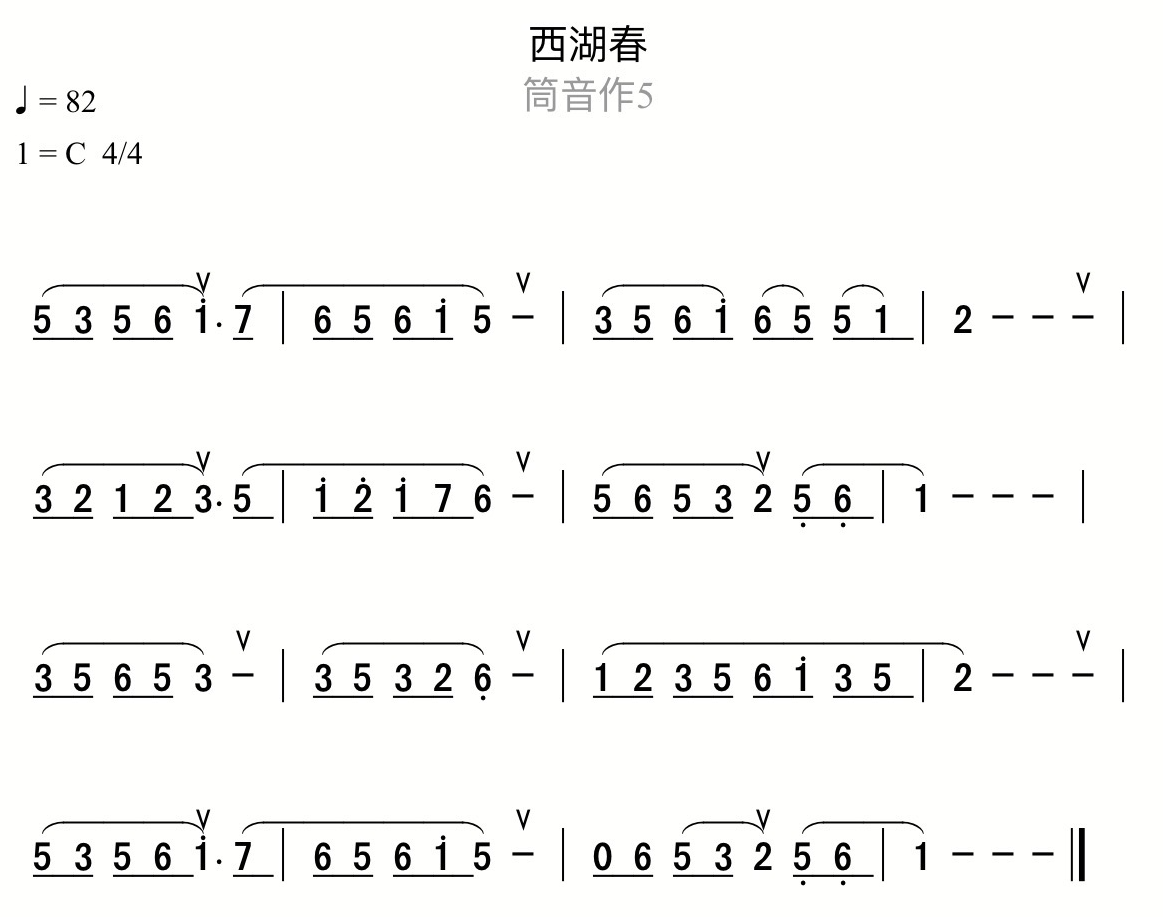
\includegraphics[width=\textwidth]{dongxiao/IMG_0860-西湖春.png} 

\section{送别}
    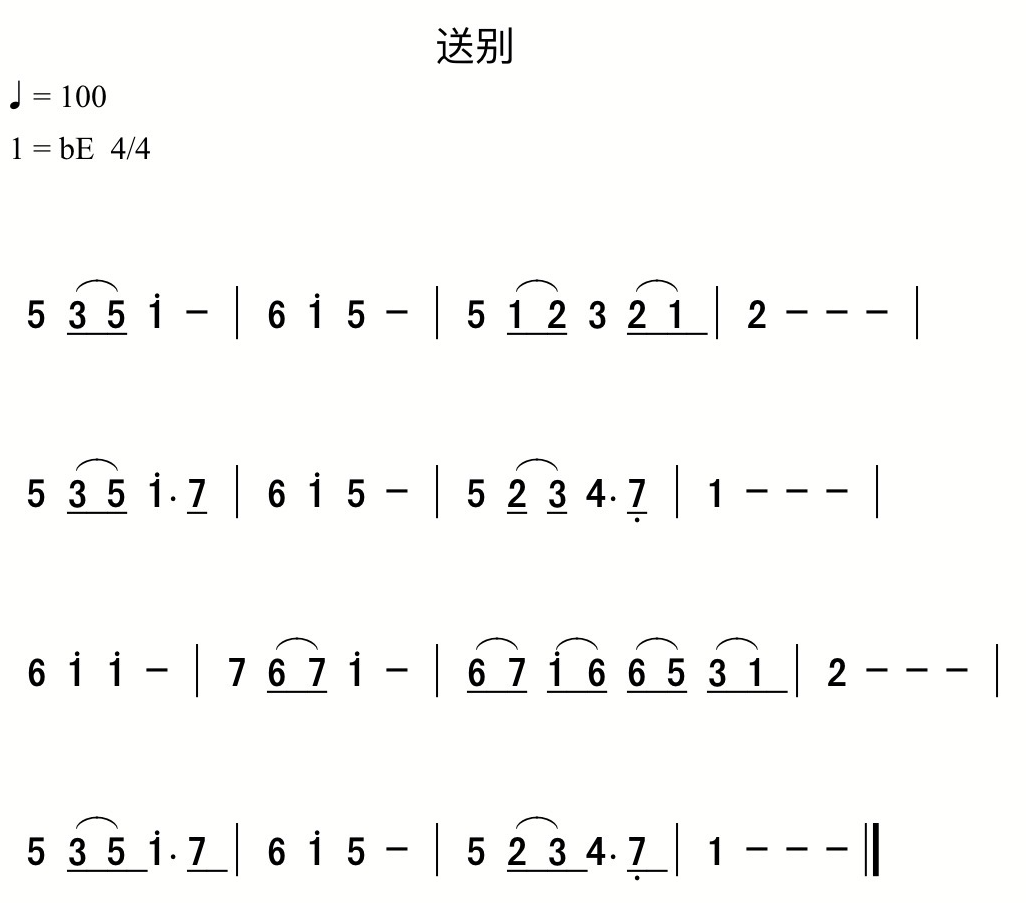
\includegraphics[width=\textwidth]{dongxiao/IMG_0855-送别.png}  
\section{苏武牧羊}
	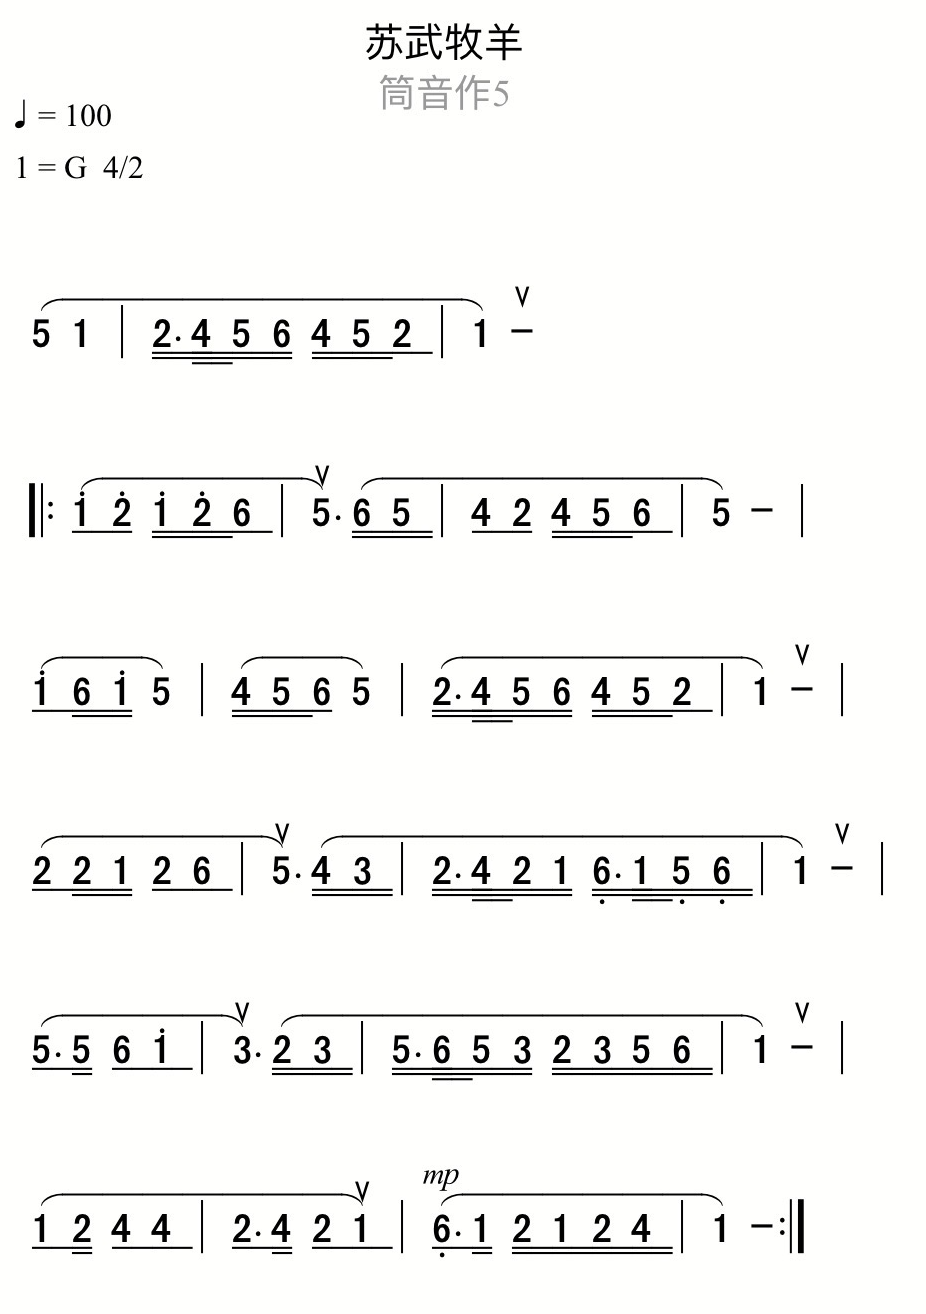
\includegraphics[width=0.9\textwidth]{dongxiao/IMG_0862-苏武牧羊.png}
\section{儿女情}          
	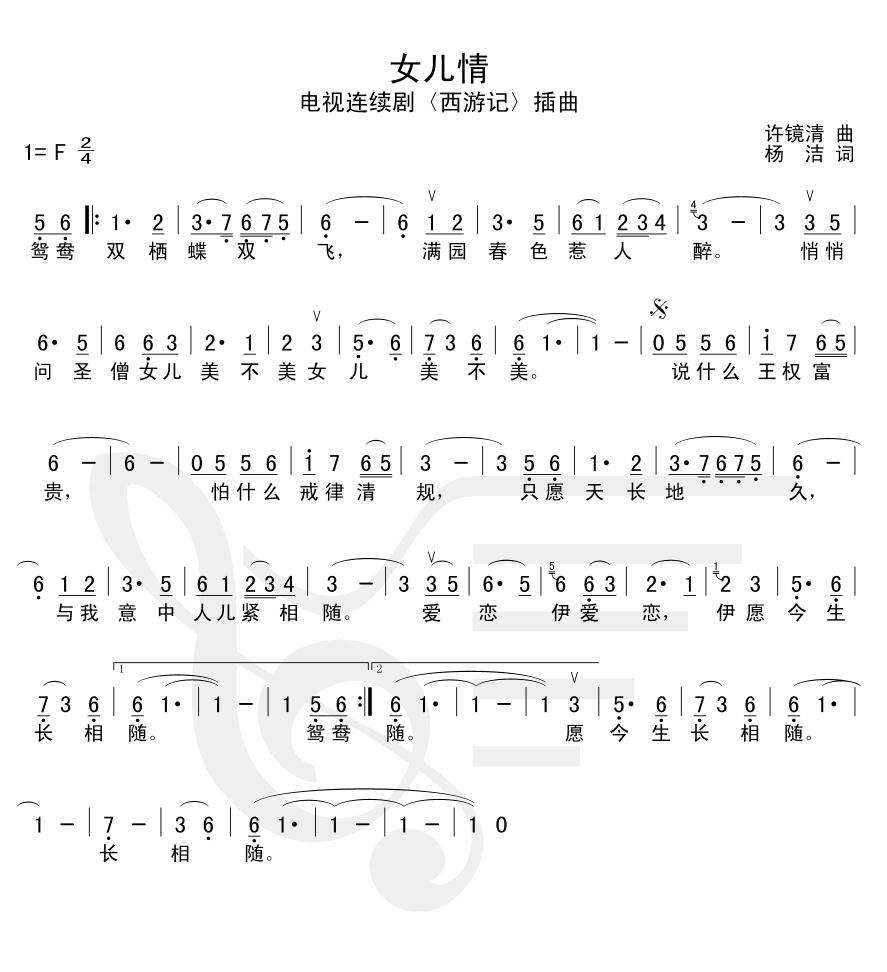
\includegraphics[width=\textwidth]{dongxiao/西游记-儿女情}  
\section{樱花}
	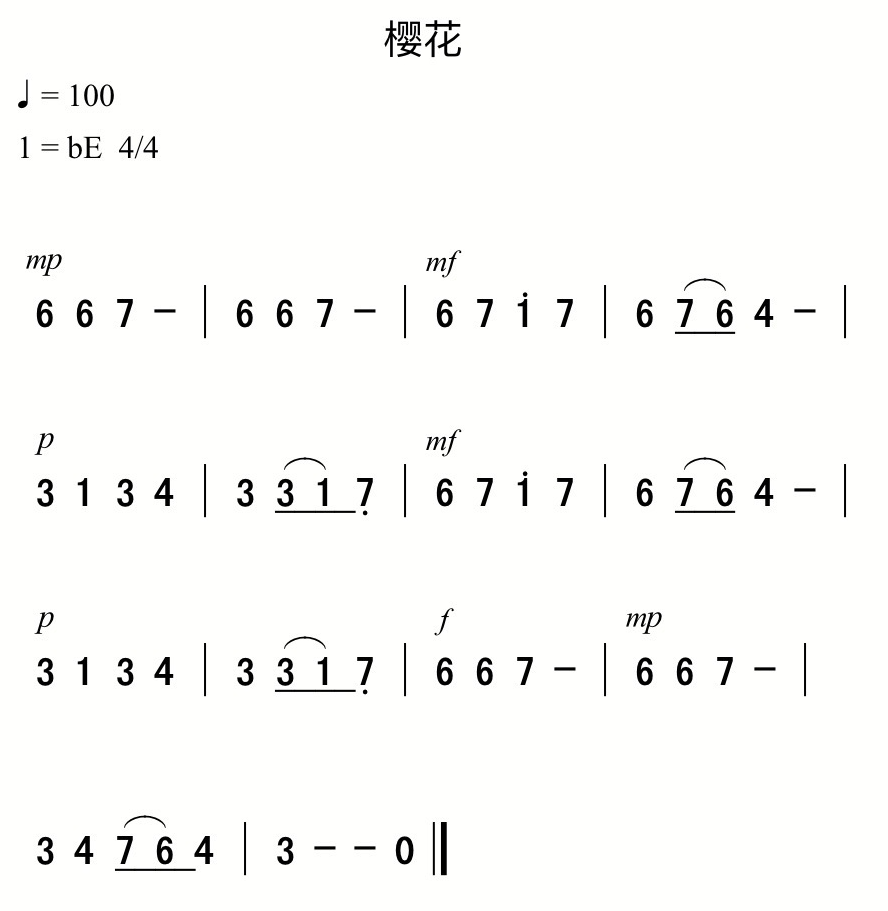
\includegraphics[width=\textwidth]{dongxiao/IMG_0861-樱花.png}  
\section{木兰辞}
	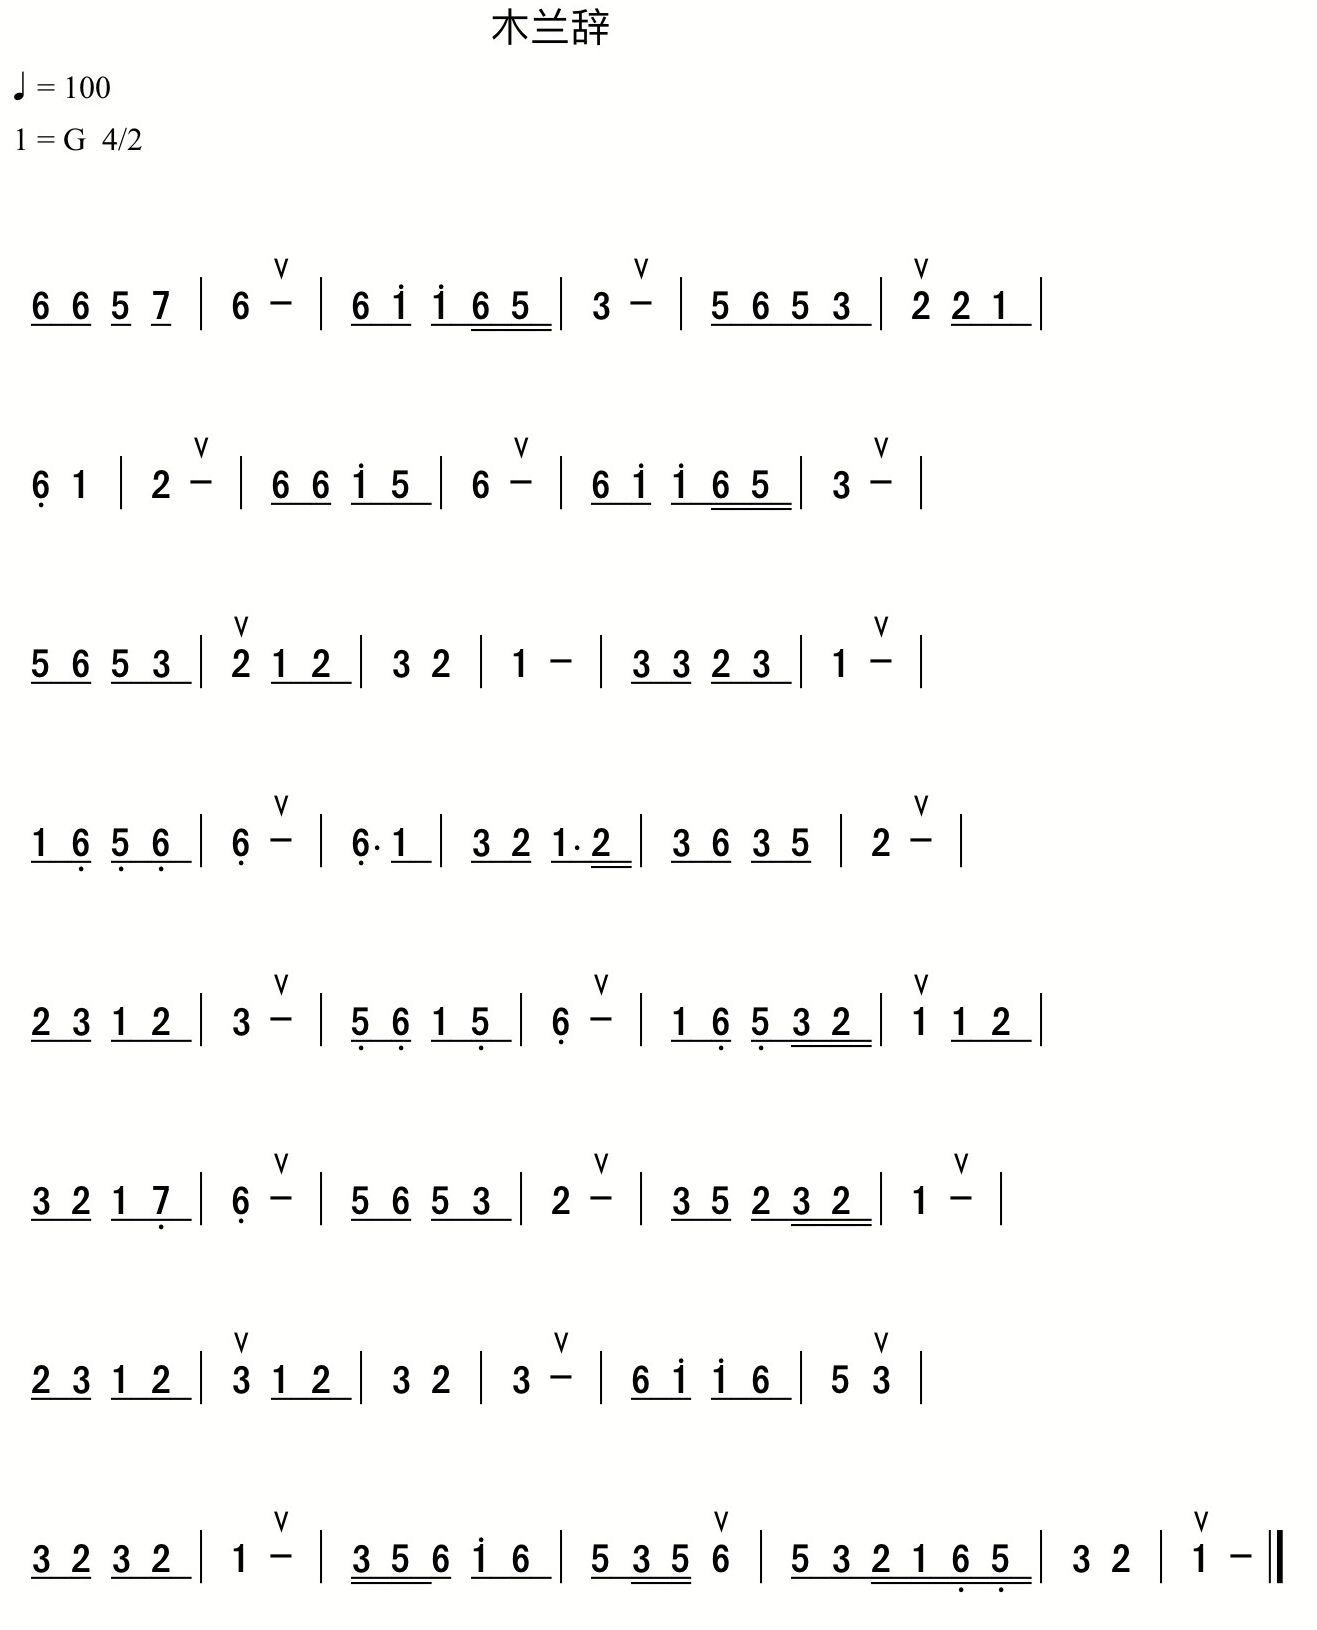
\includegraphics[width=\textwidth]{dongxiao/IMG_0867-木兰辞.png}
\section{洞箫悠悠}
    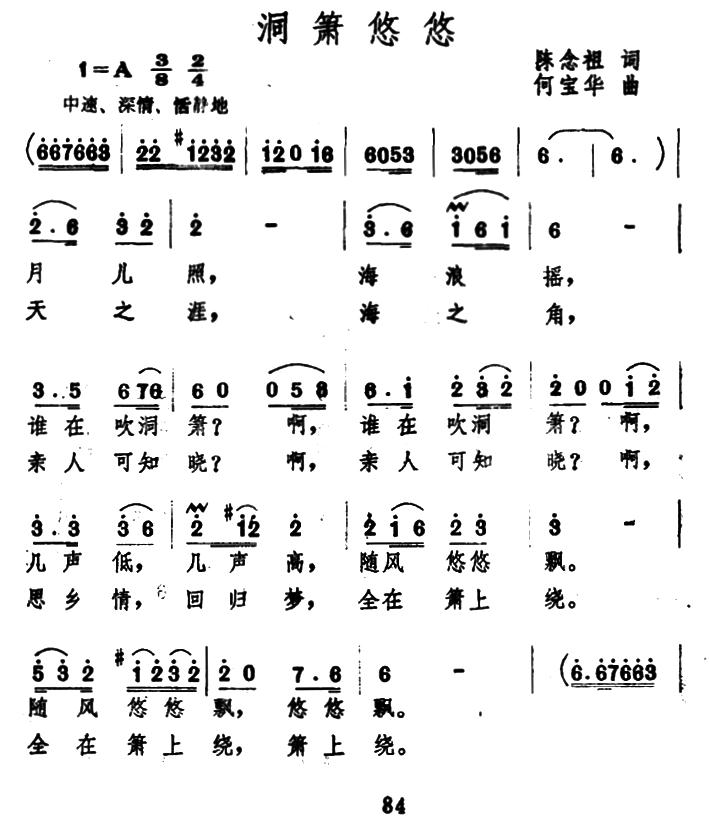
\includegraphics[width=\textwidth]{dongxiao/洞箫悠悠.jpg}
\section{玉楼春}
    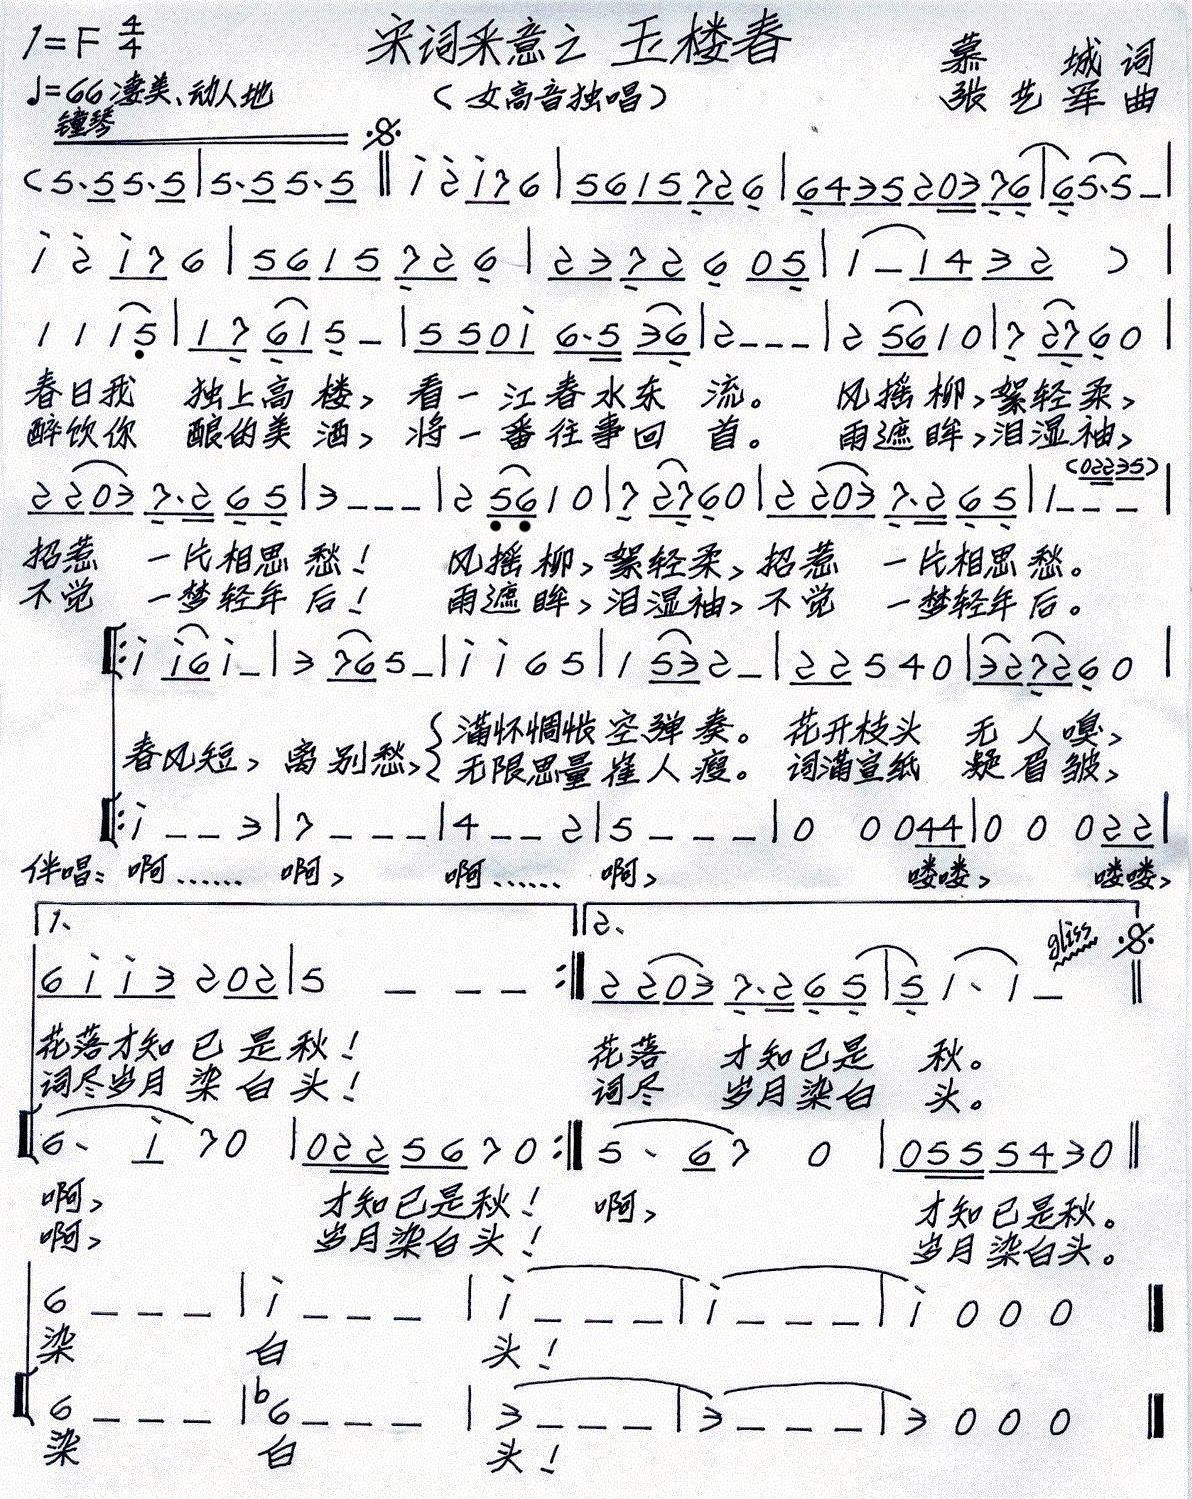
\includegraphics[width=\textwidth]{dongxiao/20200323玉楼春.jpg}
    
\section{风留念}
    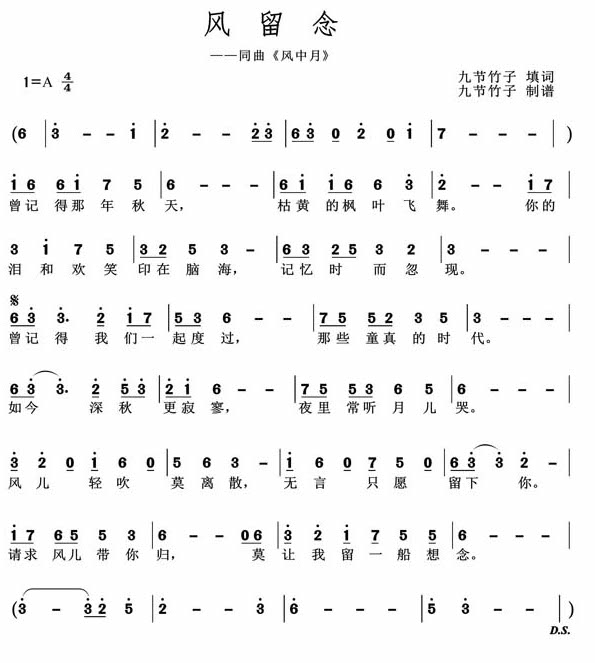
\includegraphics[width=\textwidth]{dongxiao/20200323风留念.jpg}
\section{墨香-长安曲}
    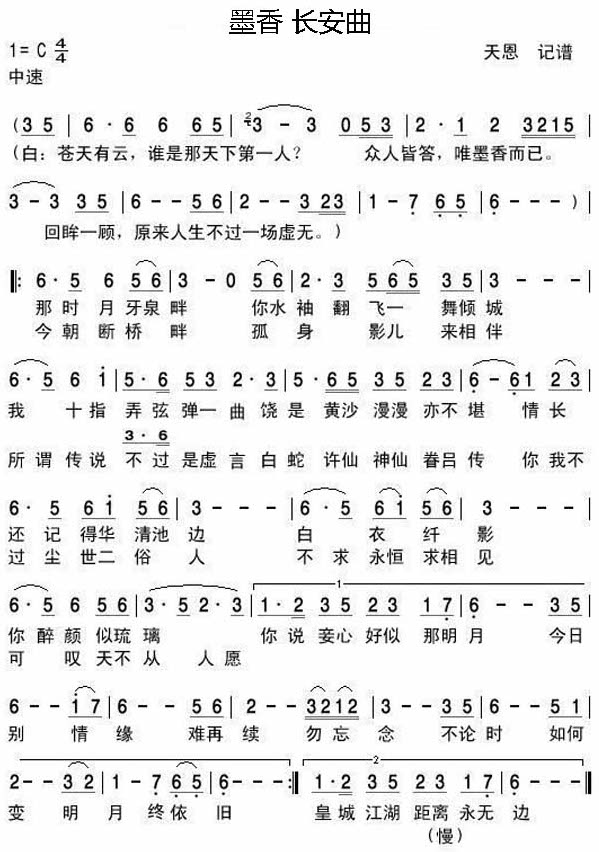
\includegraphics[width=0.9\textwidth]{dongxiao/20200323墨香-长安曲.jpg} 
\section{思美人兮}
    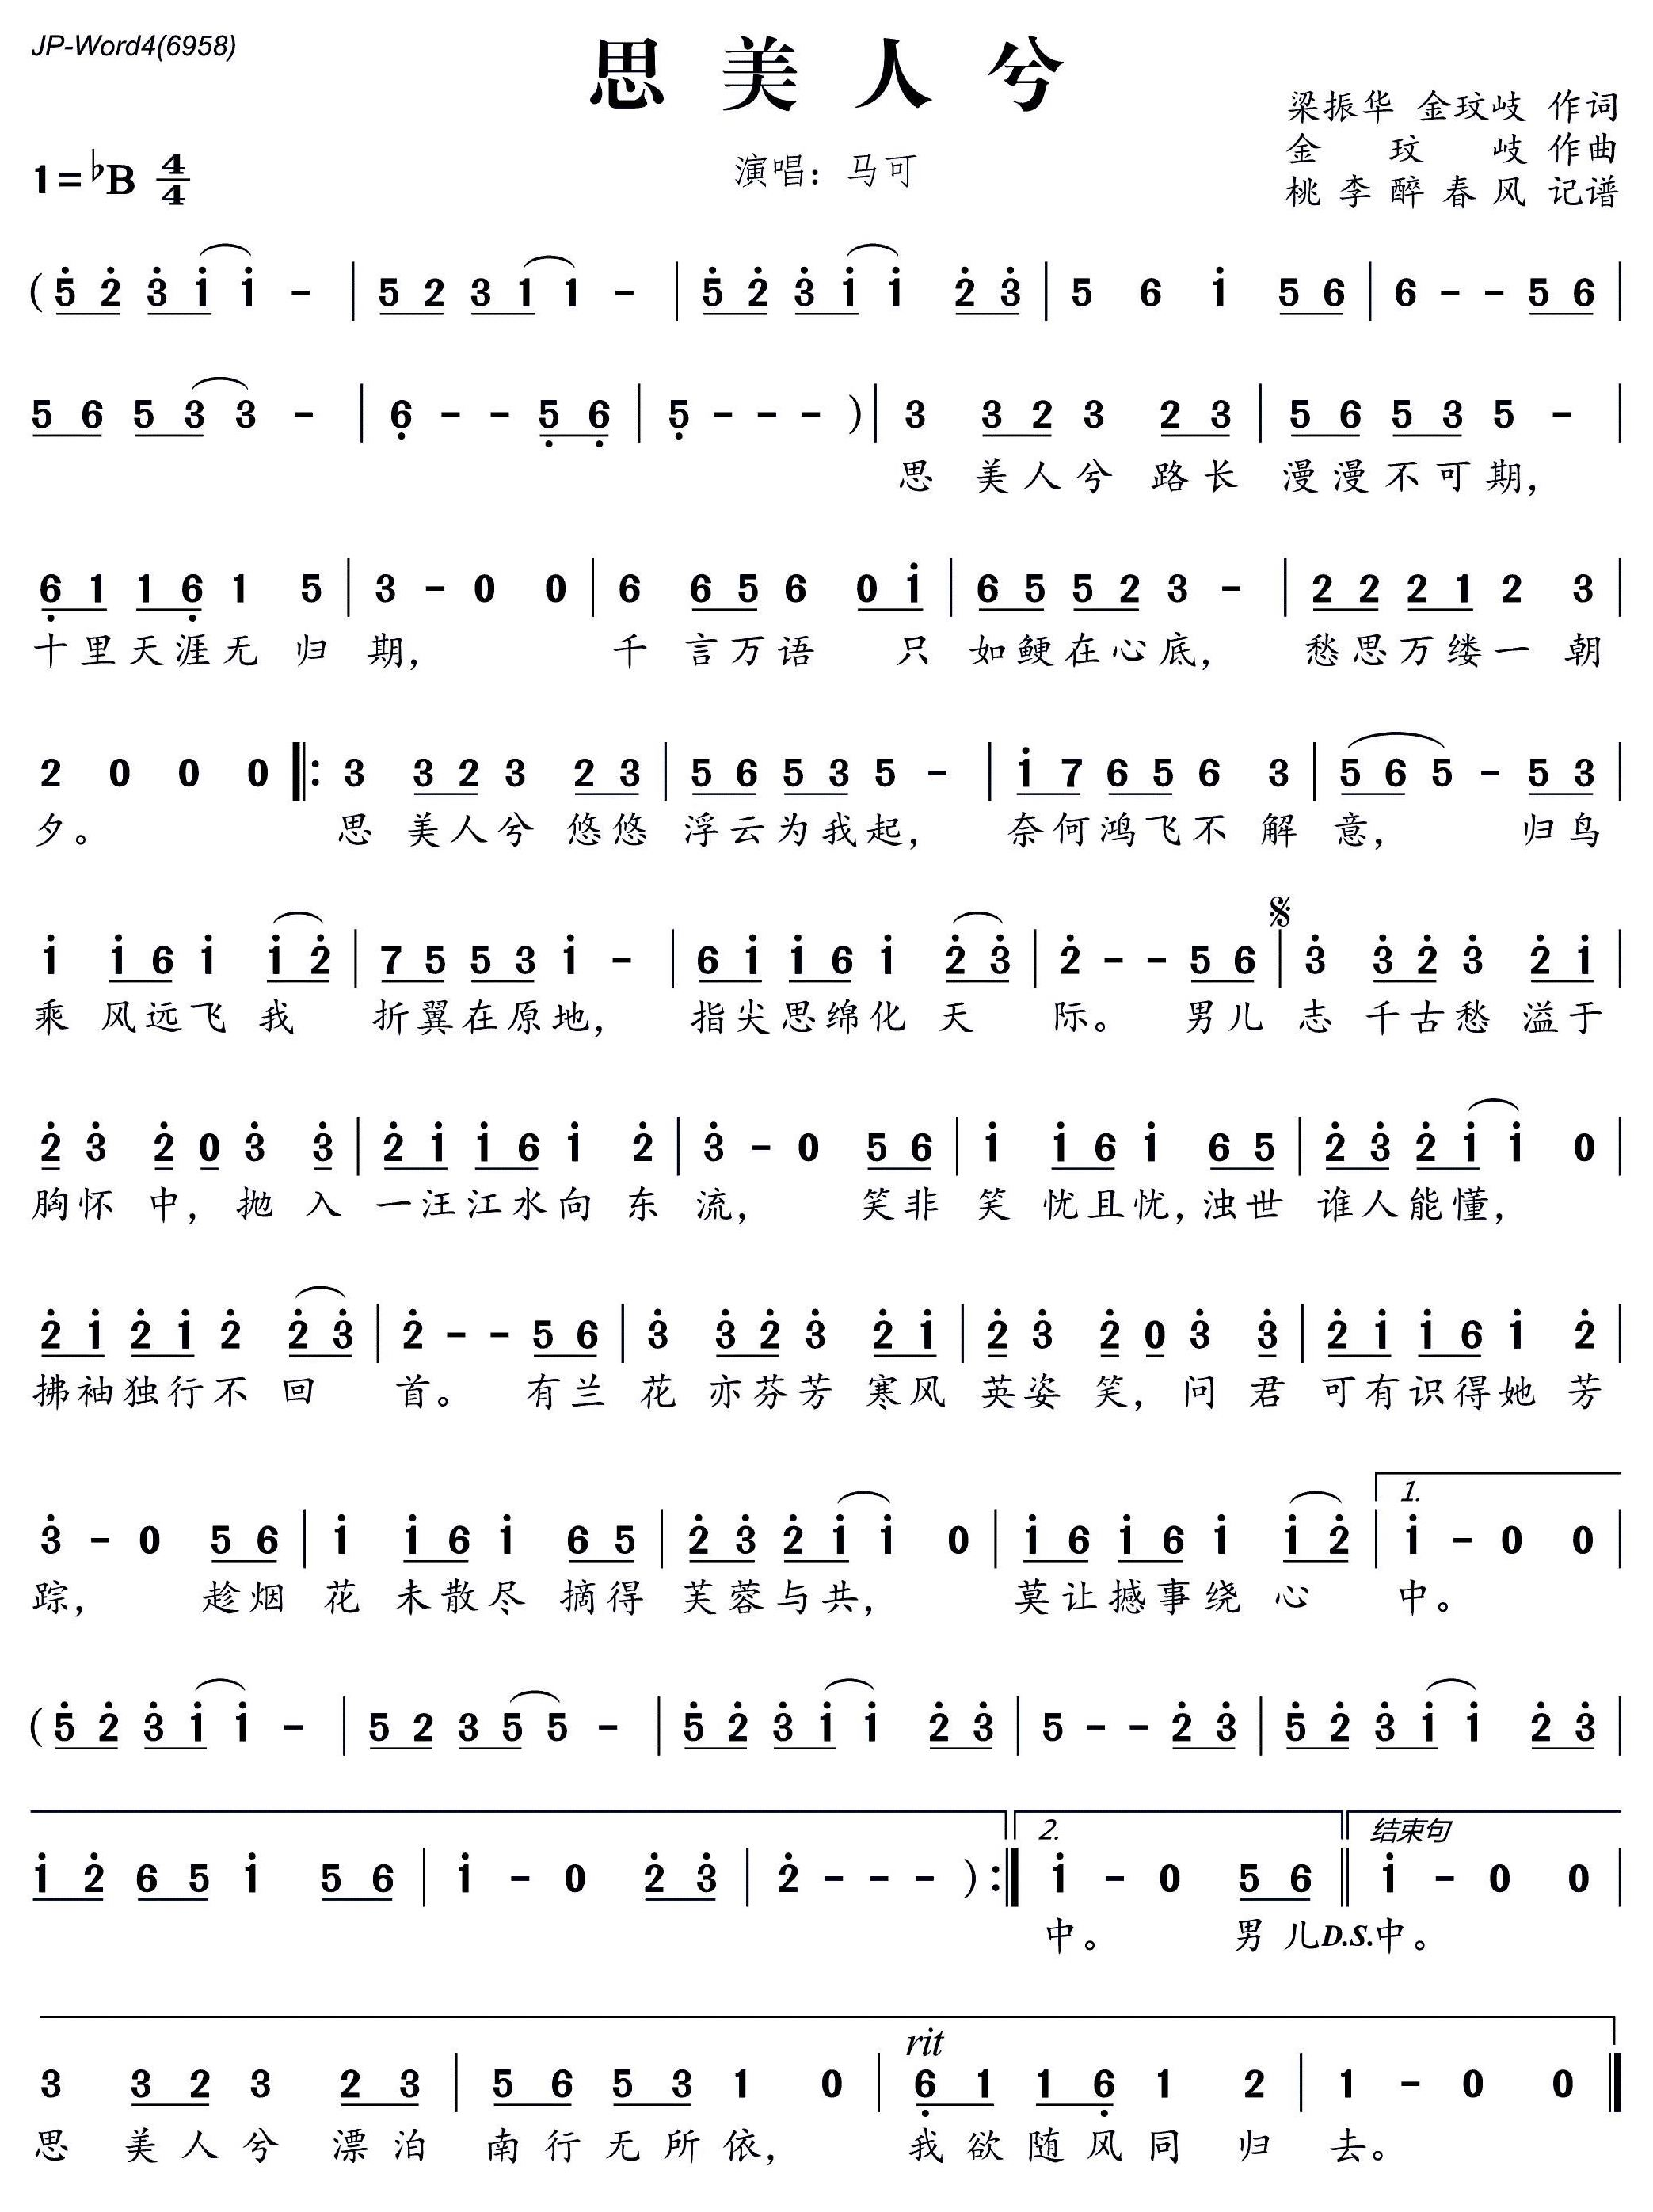
\includegraphics[width=\textwidth]{dongxiao/20200402-思美人.jpg}
\section{意难平}
    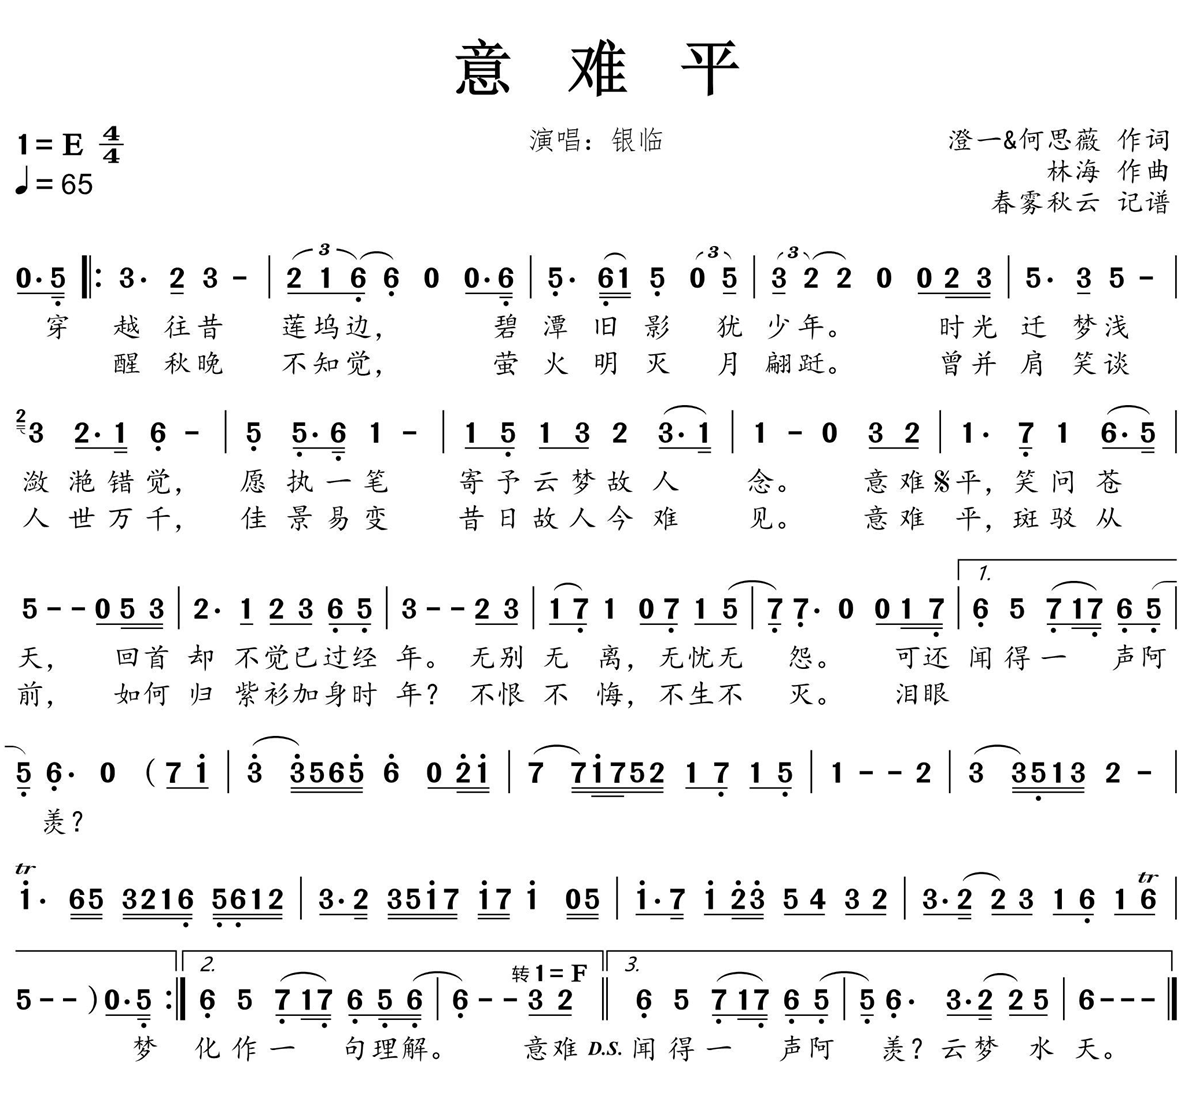
\includegraphics[width=\textwidth]{dongxiao/20200402-意难平} 
\section{城市很静}
    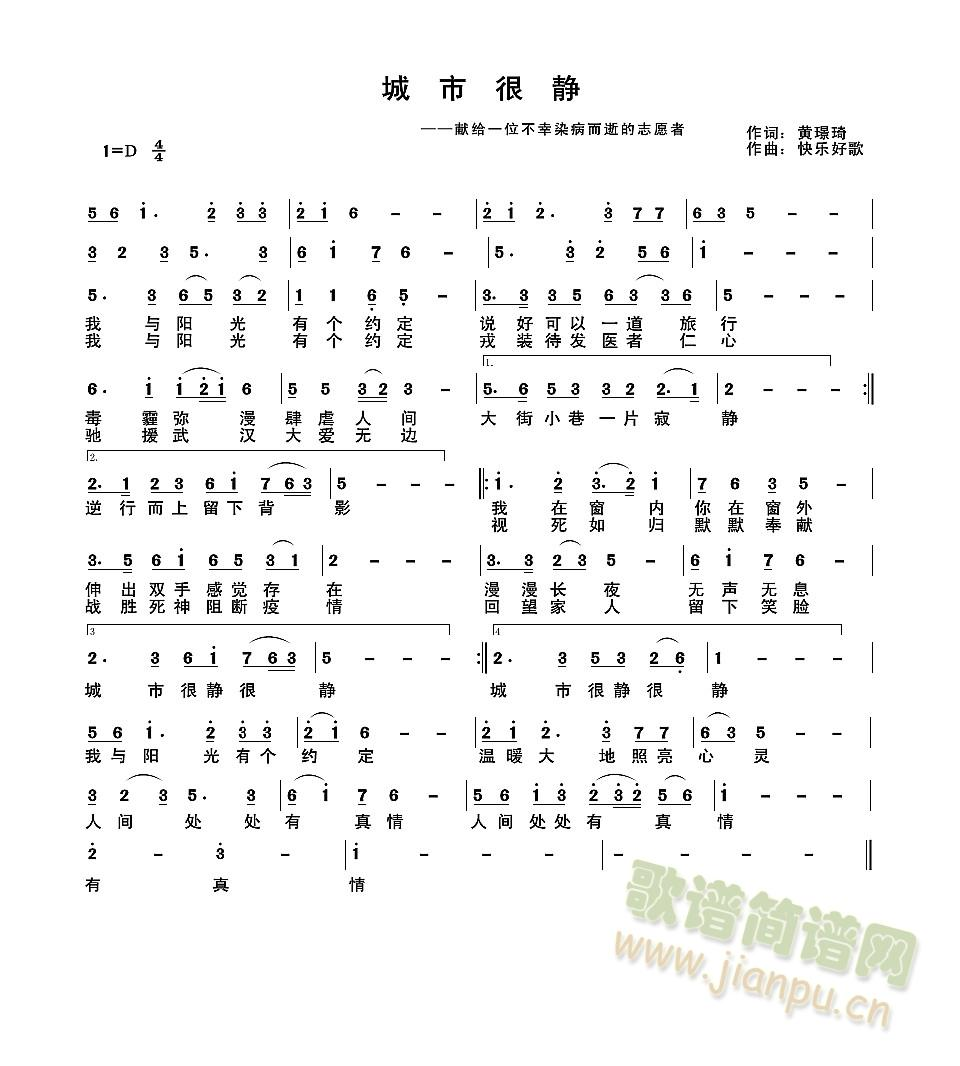
\includegraphics[width=\textwidth]{dongxiao/20200402-城市很静} 
\section{等你回家}
    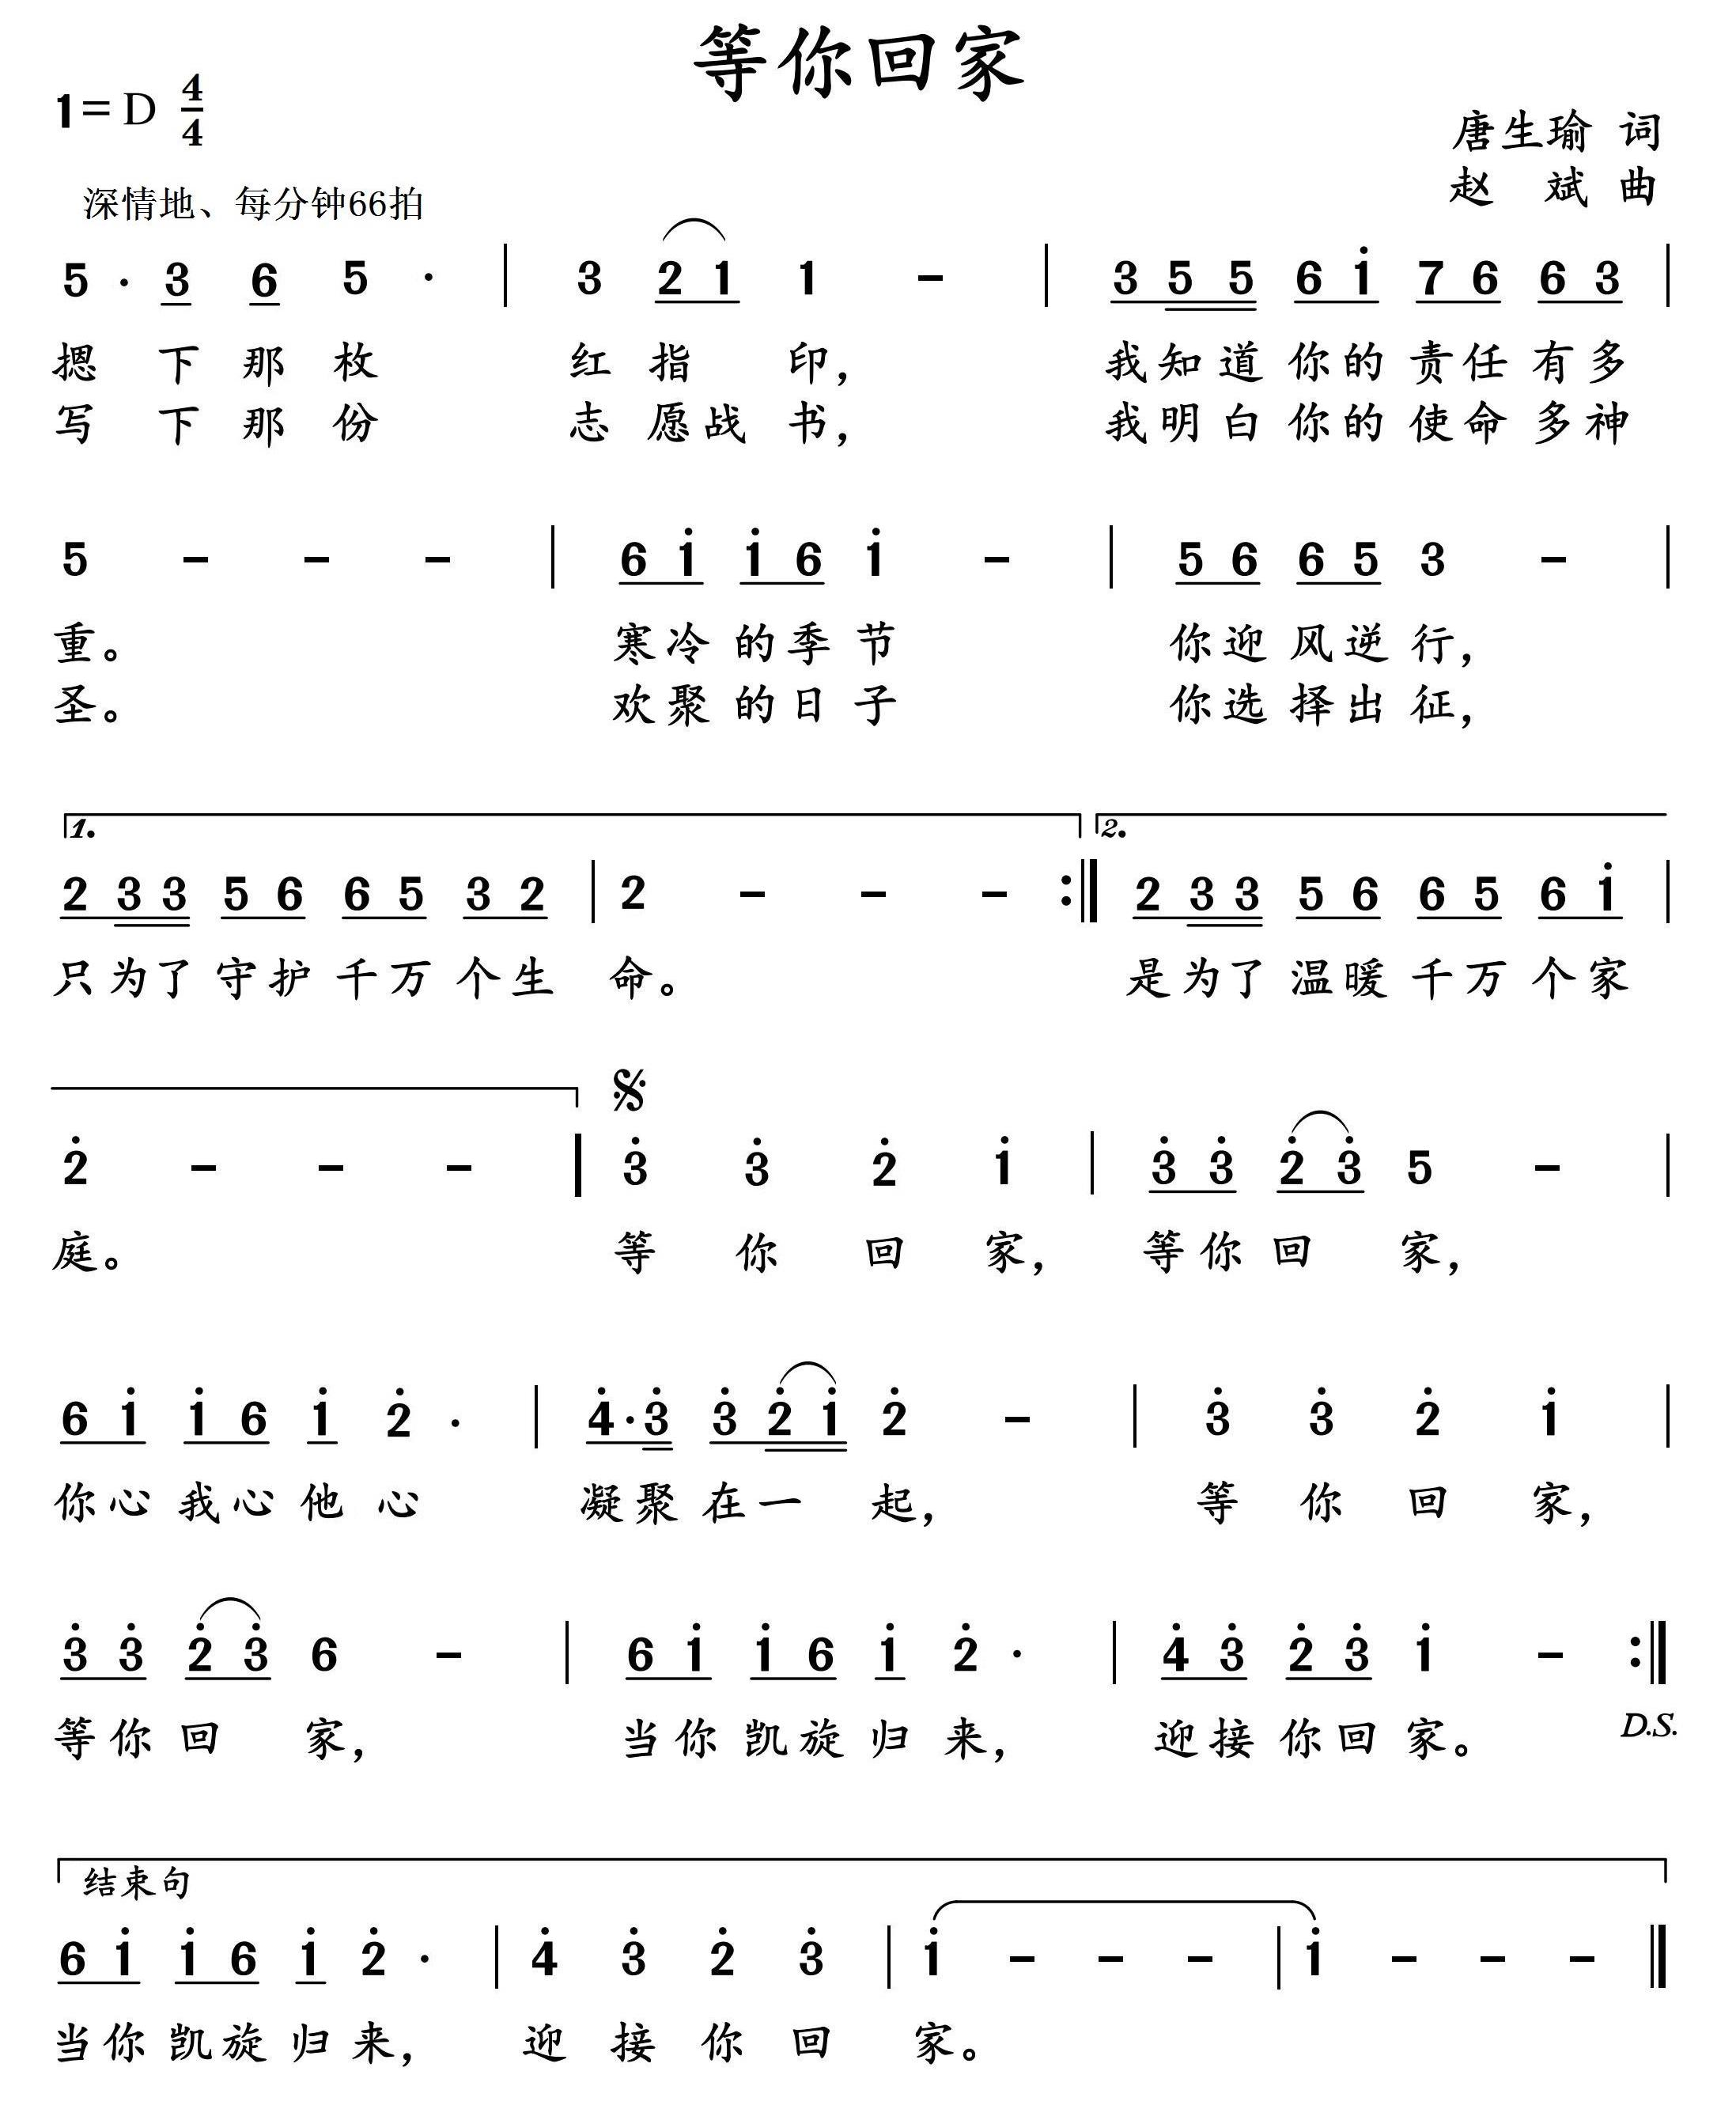
\includegraphics[width=\textwidth]{dongxiao/20200402-等你回家}

\end{document}
